%!TEX root = ..\ms-thesis.tex
\chapter{Results and Discussion} \label{ch:results-discussion}

\section{Hot Ductility Curves}
The on-heating and on-cooling hot ductility curves for the Cone~1 and Cone~5 materials are presented in Figure~\ref{fig:c1-hot-ductility} and Figure~\ref{fig:c5-hot-ductility} respectively.  In general, the on-heating ductility for both Cones increased with testing temperature, up to a ductility maximum, before dropping rapidly to zero over a short temperature range.  From Figure~\ref{fig:c1-hot-ductility} and Figure~\ref{fig:c5-hot-ductility}, it is apparent that Cone~1 and Cone~5 also showed similar trends in on-cooling behavior, in that the on-cooling ductility remains essentially zero for a definite temperature range below the \gls{zdt} before gradually increasing at lower test temperatures.  Specifically for Cone~1, it is apparent from Figure~\ref{fig:c1-hot-ductility} that the Cone~1 material exhibited an on-heating \gls{zdt} of 2375\textdegree{}F and an on-cooling DRT of 2300\textdegree{}F, resulting in an NDR of 75F\textdegree{}.  Figure~\ref{fig:c5-hot-ductility} shows that the Cone~5 material also exhibited an on-heating \gls{zdt} of 2375\textdegree{}F, DRT of 2300\textdegree{}F, and NDR of 75F\textdegree{}.  These characteristics of the hot ductility curves for both materials are summarized in Table~\ref{tab:hot-ductility-results}.

\begin{figure}[h!]
\setlength{\abovecaptionskip}{15pt}
\centering
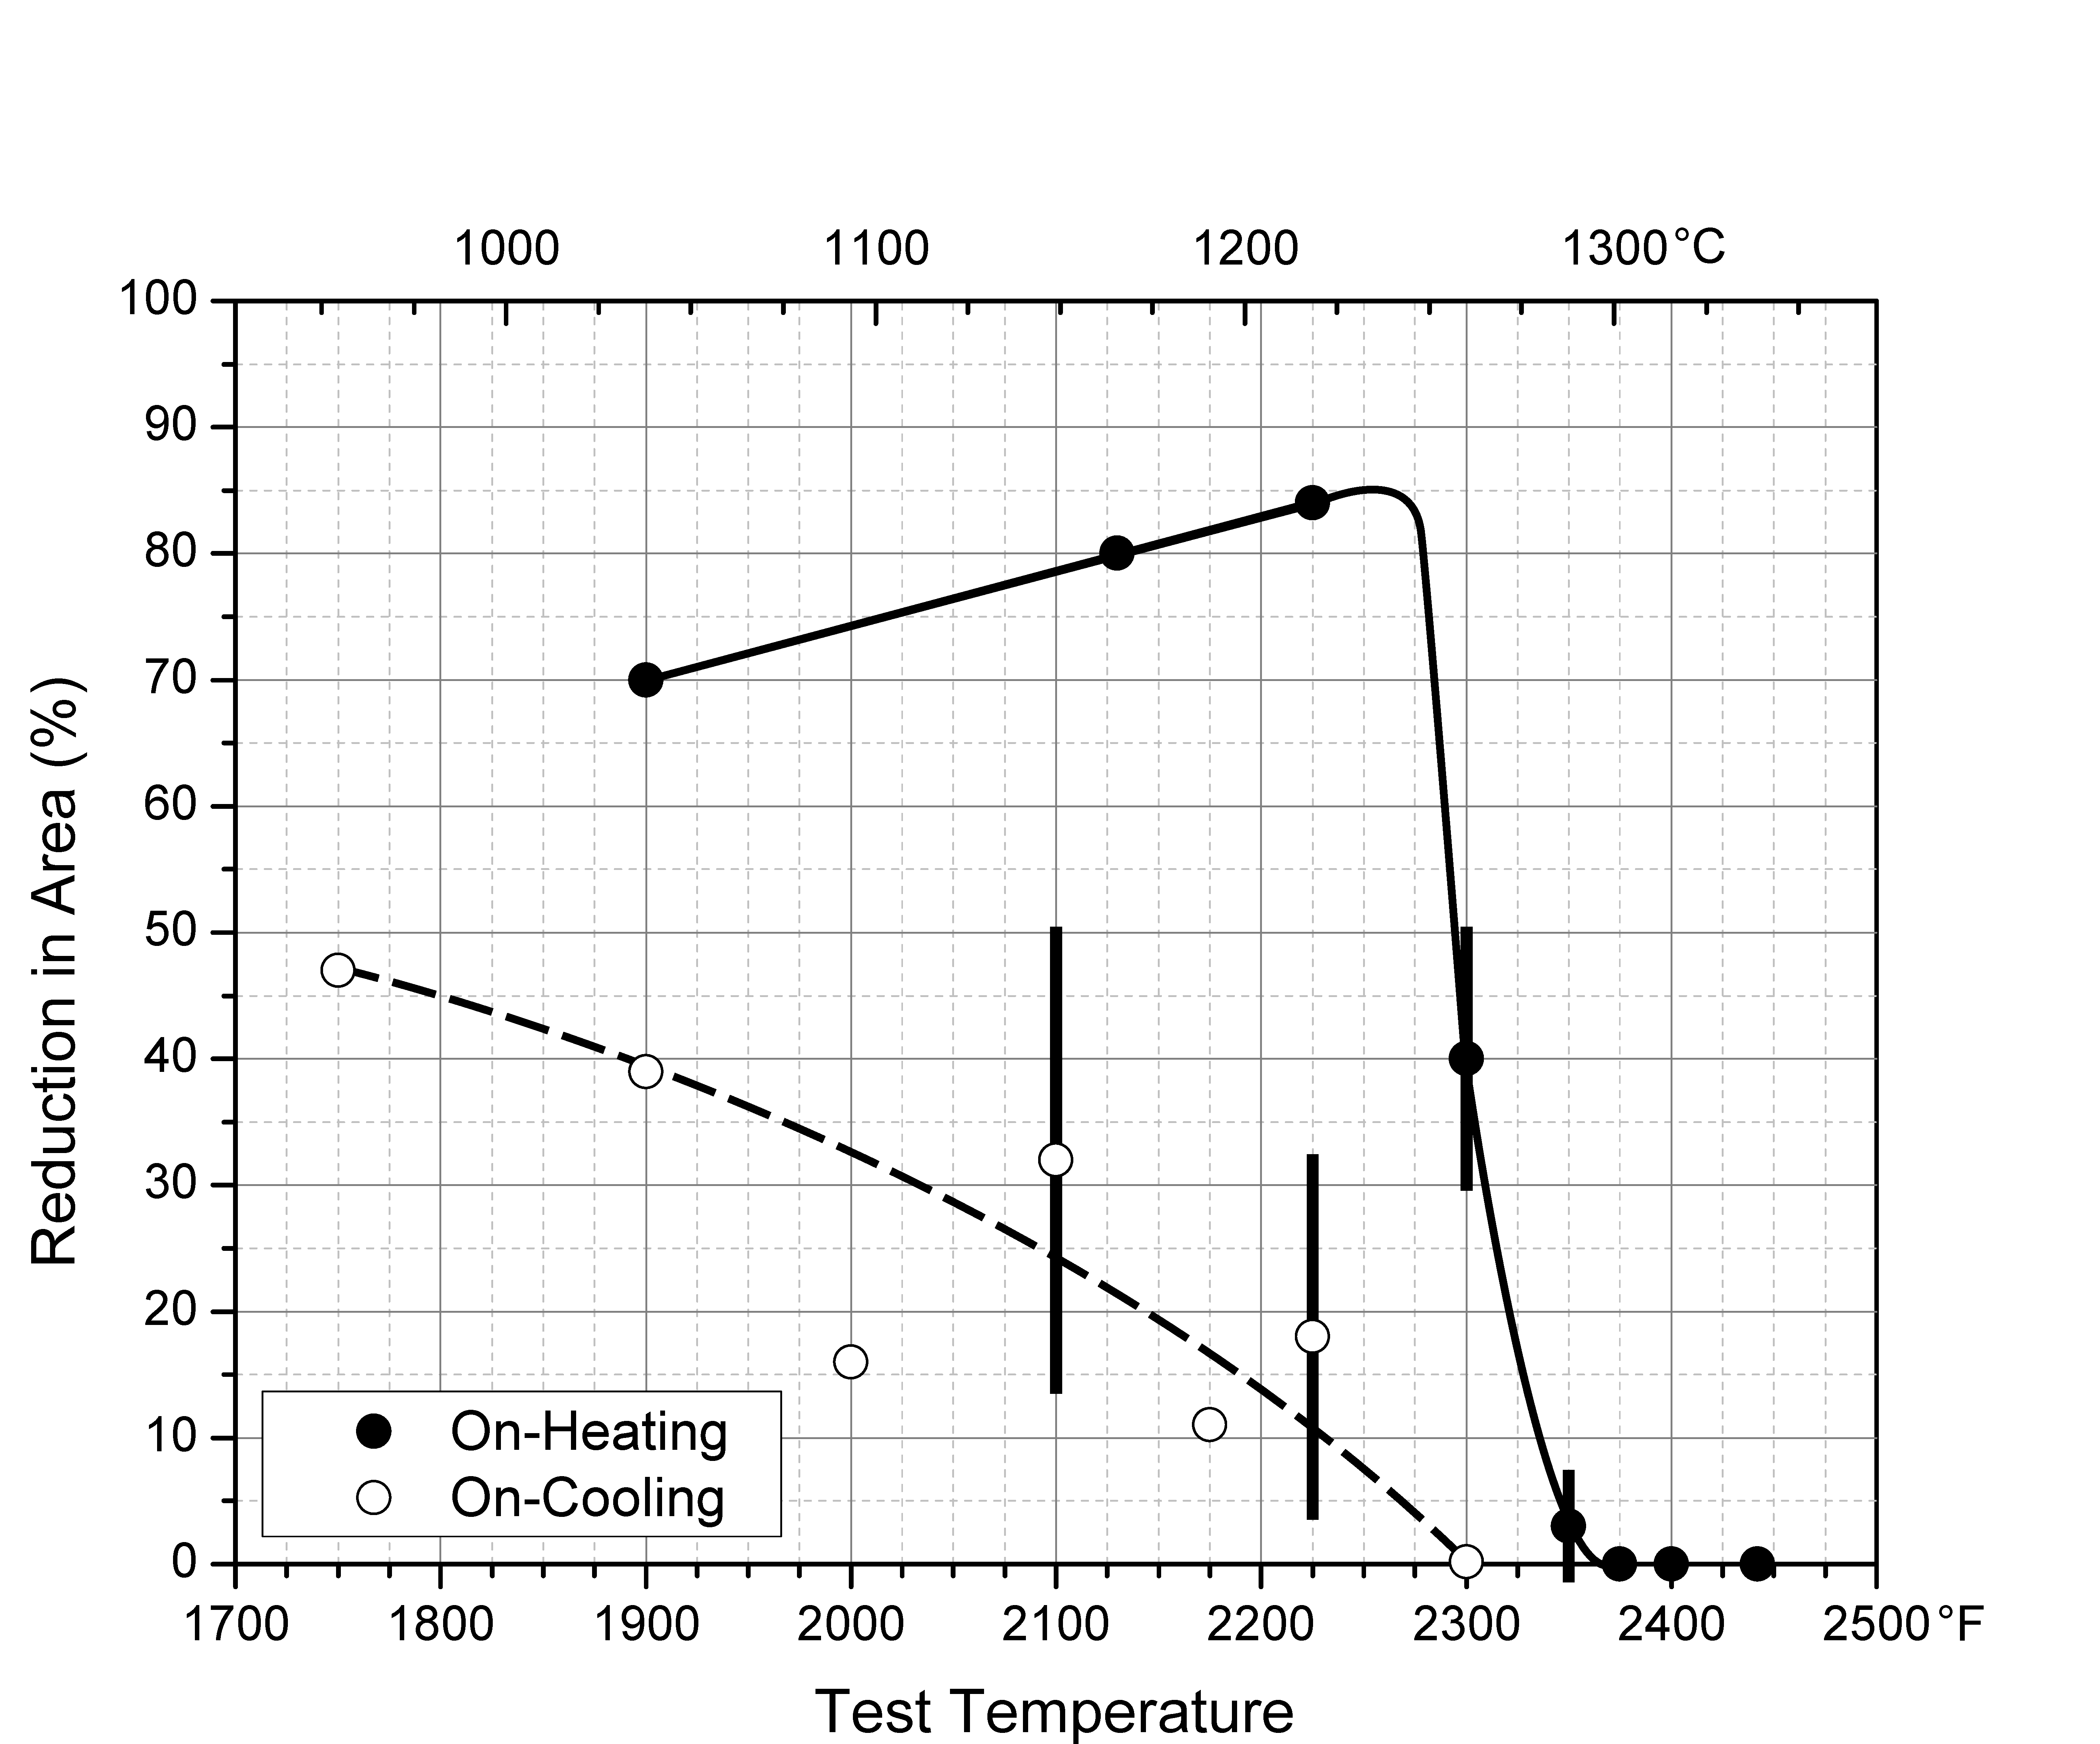
\includegraphics[width=6in]{figures/hot-ductility/c1-hot-ductility-curve.pdf}
\caption[Hot Ductility Behavior of Cone~1 Base Metal.]{Hot Ductility Behavior of CT15C Cone~1 Base Metal.  Bars indicate range of \%RA values at indicated test temperature.  On-Heating Curve Exhibits Class H1 behavior with \gls{zdt} = 2375\textdegree{}F; On-Cooling Curve (from Peak Temperature of 2375\textdegree{}F) Exhibits Class C3 behavior.  \gls{drr}(2225\textdegree{}F) = 21\%. Hot Ductility Test Parameters Given in Table~\ref{tab:hot-ductility-parameters}.}
\label{fig:c1-hot-ductility}
\end{figure}

\begin{figure}[h!]
\setlength{\abovecaptionskip}{15pt}
\centering
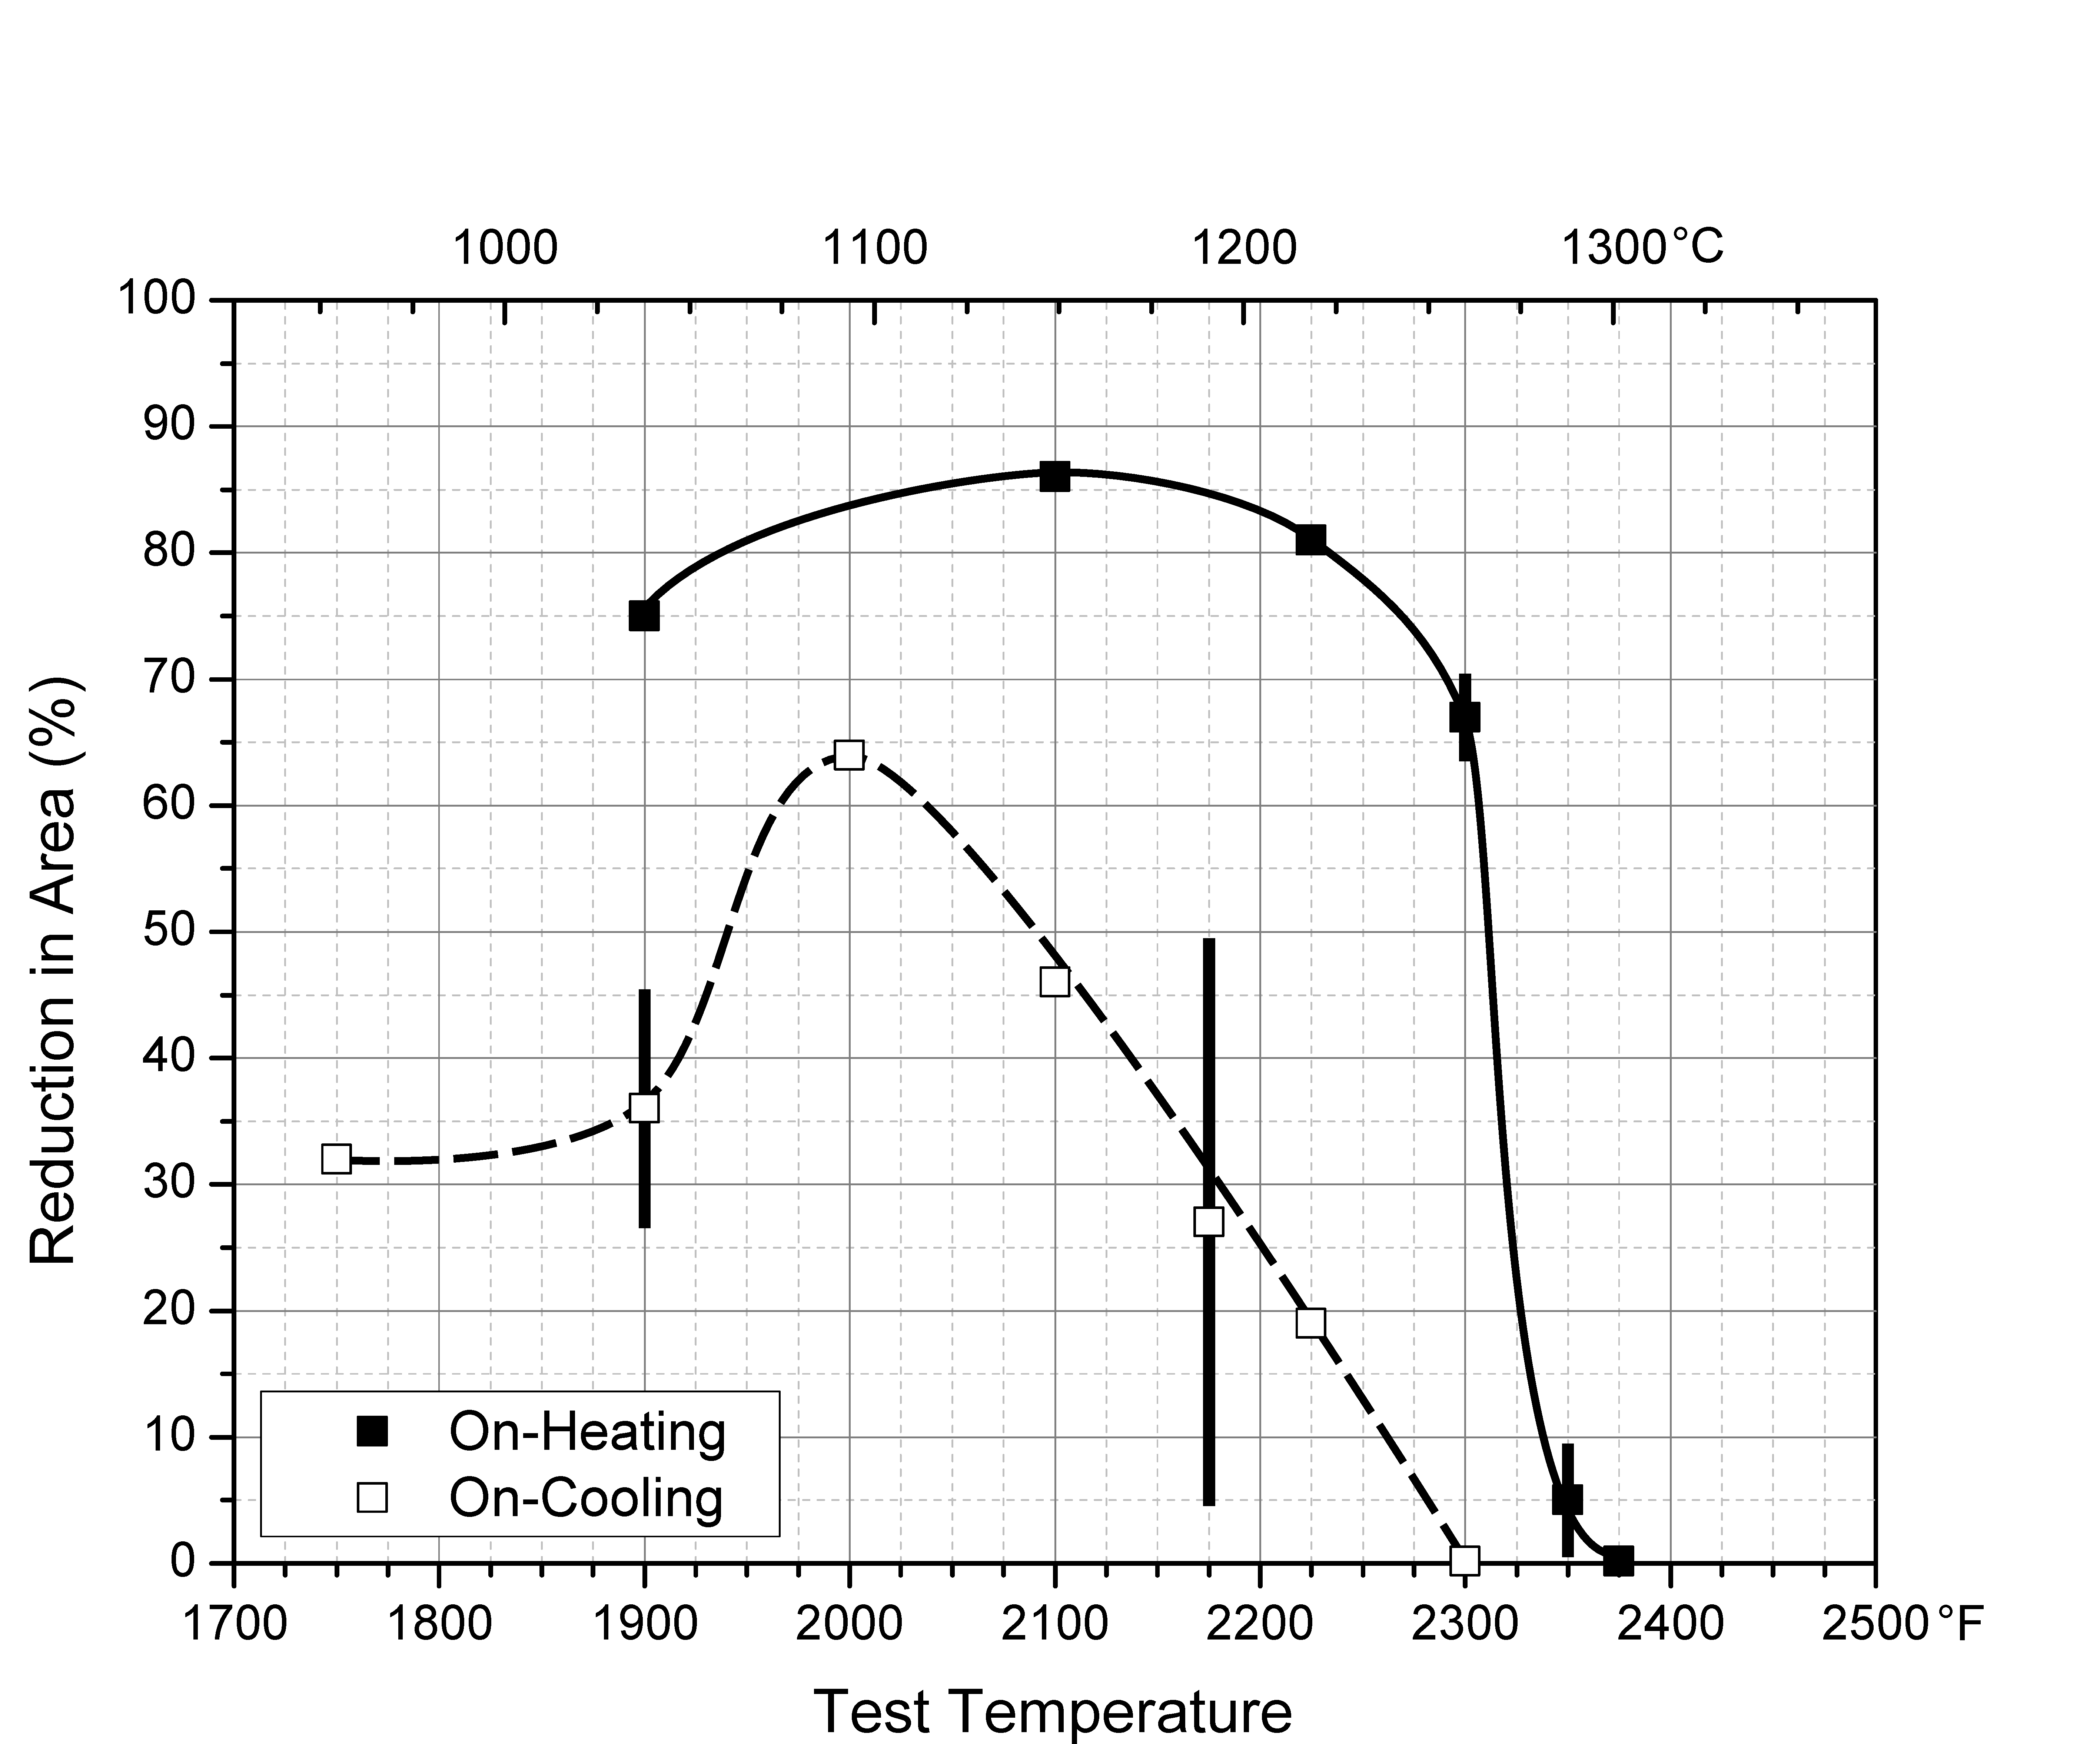
\includegraphics[width=6in]{figures/hot-ductility/c5-hot-ductility-curve.pdf}
\caption[Hot Ductility Behavior of Cone~5 Base Metal.]{Hot Ductility Behavior of CT15C Cone~5 Base Metal.  Bars indicate range of \%RA values at indicated test temperature.  On-Heating Curve Exhibits Class H1 behavior with \gls{zdt} = 2375\textdegree{}F; On-Cooling Curve (from Peak Temperature of 2375\textdegree{}F) Exhibits Class C3 behavior.  \gls{drr}(2225\textdegree{}F) = 23\%. Hot Ductility Test Parameters Given in Table~\ref{tab:hot-ductility-parameters}.}
\label{fig:c5-hot-ductility}
\end{figure}

\begin{table}[h]
\caption{Summary of hot ductility characteristics for Cone~1 and Cone~5 materials, as determined from the curves in Figure~\ref{fig:c1-hot-ductility} and Figure~\ref{fig:c5-hot-ductility}.}
\begin{tabular}{ lccc }
\toprule
\textbf{Material ID and Condition} & \textbf{\gls{zdt} (F)} & \textbf{DRT (F)} & \textbf{NDR (\gls{zdt}-DRT) (F)} \\
\midrule
Cone~1 (Service-Exposed) & 2375 & 2300 & 75 \\
Cone~5 (Nominally solution-annealed) & 2375 & 2300 & 75 \\
\bottomrule
\end{tabular}
\label{tab:hot-ductility-results}
\end{table}



As can be seen from Figure~\ref{fig:c1-hot-ductility} and Figure~\ref{fig:c5-hot-ductility}, the on-heating hot ductility curves for both Cone materials appear similar, with similar reduction in area (\% RA) values at each test temperature, except in the vicinity of 2300\textdegree{}F.  At this temperature, Cone~1 exhibits a more rapid loss in ductility than Cone~5.  Based on the Nippes evaluation criteria \cite{nippes_further_1957} described previously, examination of the shape of the on-heating ductility curves in Figure~\ref{fig:c1-hot-ductility} and Figure~\ref{fig:c5-hot-ductility} shows that both Cones exhibit Class H1 on-heating hot ductility behavior rather than Class H2 behavior.  This observation regarding the Cone~1 and Cone~5 materials is indeterminate on its own, as \citet{nippes_further_1957} observed in some cases that two materials which both showed H1 on-heating behavior were later found to exhibit either crack-sensitive or crack-insensitive characteristics when tested on-cooling.

The on-cooling ductility curves for the Cone~1 and Cone~5 materials after exposure to a peak temperature corresponding to the on-heating \gls{zdt} (2375\textdegree{}F) are also given in Figure~\ref{fig:c1-hot-ductility} and Figure~\ref{fig:c5-hot-ductility}.  Considering the shapes of the on-cooling ductility curves, it is apparent that both Cone materials exhibit Class C3 on-cooling behavior when exposed to the \gls{zdt}, based on the Nippes criteria (Figure~\ref{fig:nippes-criteria}).  This category of on-cooling behavior is associated with the greatest degree of hot cracking susceptibility as established by \citet{nippes_further_1957}.  While in general both materials exhibit Class C3 behavior, it appears from Figure~\ref{fig:c1-hot-ductility} and Figure~\ref{fig:c5-hot-ductility} that Cone~5 shows a slightly better qualitative recovery of on-cooling ductility than Cone~1.  As shown in Figure~\ref{fig:c5-hot-ductility}, the on-cooling ductility for Cone~5 recovers to higher values than for Cone~1, particularly at 2100\textdegree{}F and 2000\textdegree{}F.  However, when considering the apparent difference, it should be noted that both Cones are cast components with a large dendrite size, and it was observed in early work on hot ductility by \citet{nippes_further_1957} that castings typically showed wider variation in ductility values at a given test temperature than was observed for wrought material.  The 20Cr-32Ni-1Nb cast material used in both Cones is no different in this regard, for example as evidenced by the variation at 2100\textdegree{}F on-cooling for Cone~1 and 2175\textdegree{}F on-cooling for Cone~5.  Due to the reality of variations in ductility values, it is recommended practice (\citet{lundin_standardization_1990_experiment}) to run a minimum of two hot ductility tests at each temperature, with some studies (\citet{nippes_further_1957}) running up to four tests per temperature for cast materials.  Unfortunately, the number of samples available in the current study was not sufficient to permit duplicate tests at all test temperatures; however, duplicates were performed wherever possible, including at the \gls{zdt}.  If sufficient samples had been available for duplicate tests at all temperatures, it is possible that the average \% RA at certain test temperatures (e.g. 2000\textdegree{}F on-cooling and 2100\textdegree{}F on-cooling) would be closer in magnitude between Cone~1 and Cone~5.  Taking these considerations into account, it is likely that Cone~1 and Cone~5 are more similar in on-cooling behavior than would be suggested by a casual inspection of the curves in Figure~\ref{fig:c1-hot-ductility} and Figure~\ref{fig:c5-hot-ductility}.

To quantify the severity of the on-cooling ductility loss exhibited by both materials, the ductility recovery rate (\gls{drr}) was determined for both Cone~1 (Figure~\ref{fig:c1-hot-ductility}) and Cone~5 (Figure~\ref{fig:c5-hot-ductility}) at a test temperature of 2225\textdegree{}F since this corresponds most closely with the observed rapid-ductility-decrease temperature (on-heating) for both Cones.  The \gls{drr} at 2225\textdegree{}F was similarly low for both Cone materials: 21\% for Cone~1 and 23\% for Cone~5.  Additionally, both Cones exhibited a region of zero on-cooling ductility (a \gls{zdr}) after exposure to the on-heating \gls{zdt}; for both Cone~1 and Cone~5, the \gls{zdr} is 75F\textdegree{} wide (2300–2375\textdegree{}F).  Considered together, the occurrence of Class C3 cooling behavior, the relatively low \gls{drr} values, and the presence of a significant \gls{zdr} all indicate that the Cone~1 and Cone~5 materials are both susceptible to hot cracking when exposed to temperatures typically experienced during a welding thermal cycle.



\section{Mictrostructure Characterization}
Optical micrographs showing typical as-received microstructures for the Cone~1 and Cone~5 materials, respectively, are presented in Figure~\ref{fig:c1-asreceived} and Figure~\ref{fig:c5-asreceived}.  Both Cone materials exhibited a cast, dendritic structure with a large dendrite size.  The higher magnification micrographs in Figure~\ref{subfig:c1-asreceived-500X} and Figure~\ref{subfig:c5-asreceived-500X} show the presence of a significant amount of fine intradendritic precipitates in addition to the larger interdendritic phases.

Optical micrographs obtained from the Cone~5 On-Heating 2375\textdegree{}F (\gls{zdt}) sample are presented in Figure~\ref{fig:c5-oh-2375} and show the region adjacent to the fracture surface.  It is apparent from Figure~\ref{subfig:c5-oh-2375-50X} that the crack paths follow the interdendritic boundaries and that the greatest extent of crack opening along the boundaries generally occurs perpendicular to the hot ductility test tensile loading direction (also visible in Figure~\ref{subfig:c5-oh-2375-200X}).  A region of the Cone~5 On-Heating 2375\textdegree{}F (\gls{zdt}) sample which was remote from the fracture location (not subjected to the simulated thermal cycle) is shown in Figure~\ref{fig:c5-oh-2375-remote}.  Comparing Figure~\ref{subfig:c5-oh-2375-500X} and Figure~\ref{subfig:c5-oh-2375-remote-500x}, it is apparent that the extent of intradendritic precipitates is reduced in the vicinity of the fracture surface.

\begin{figure}
\centering
\subfloat[100X]{\label{subfig:c1-asreceived-100X}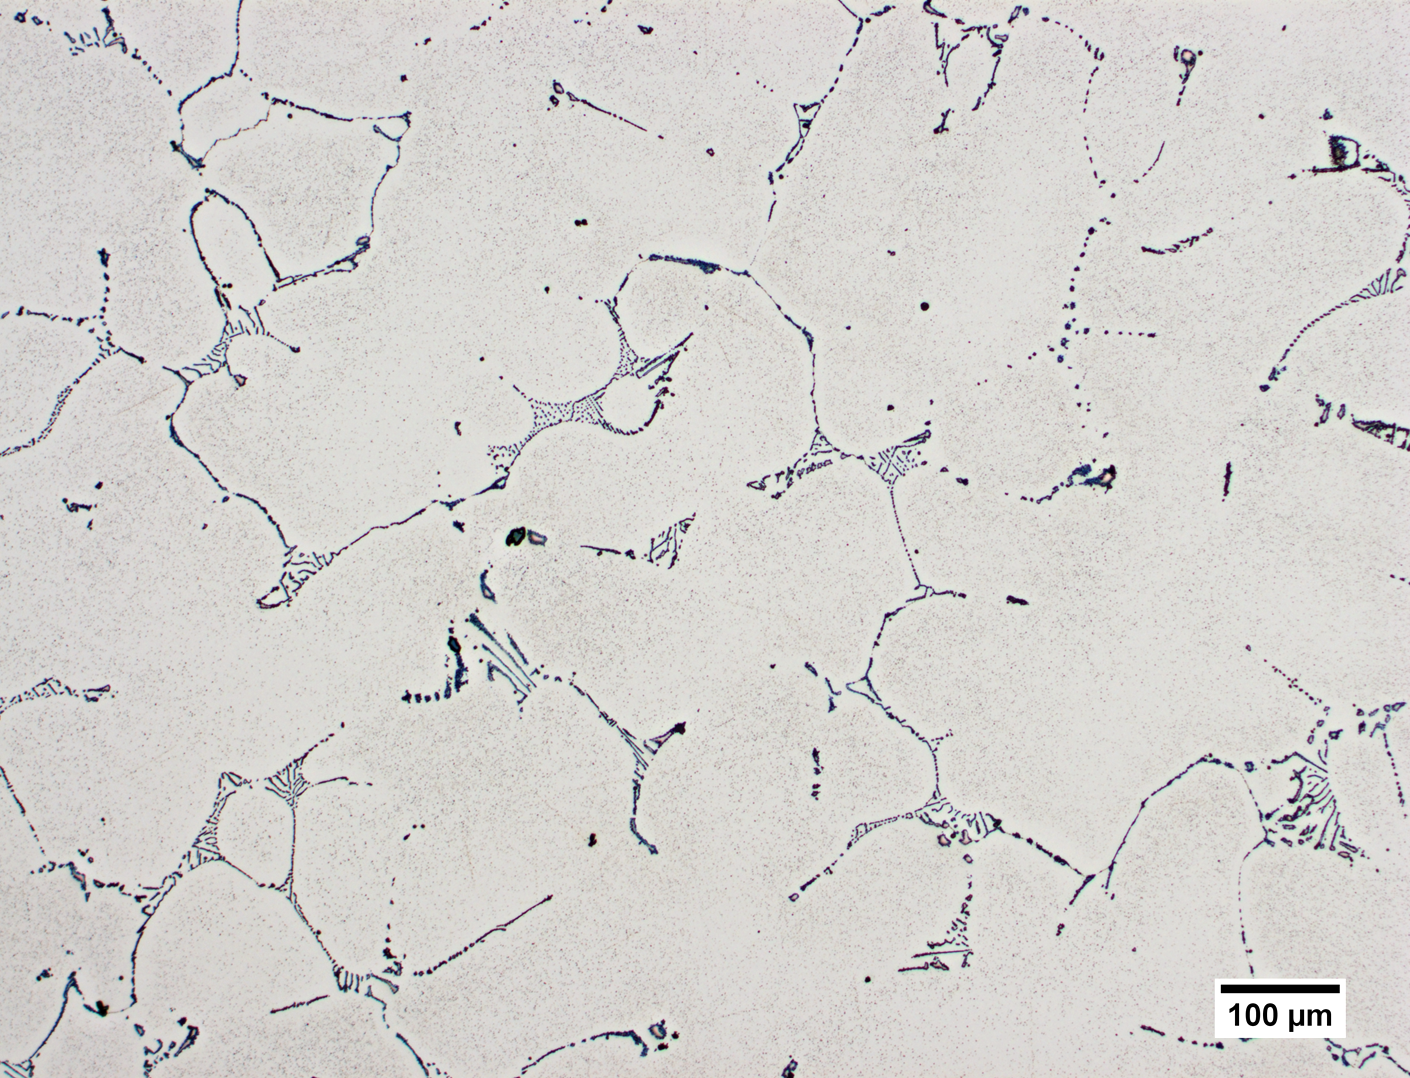
\includegraphics[width=4.7in]{figures/hot-ductility/c1-ar-100X}}

\subfloat[500X]{\label{subfig:c1-asreceived-500X}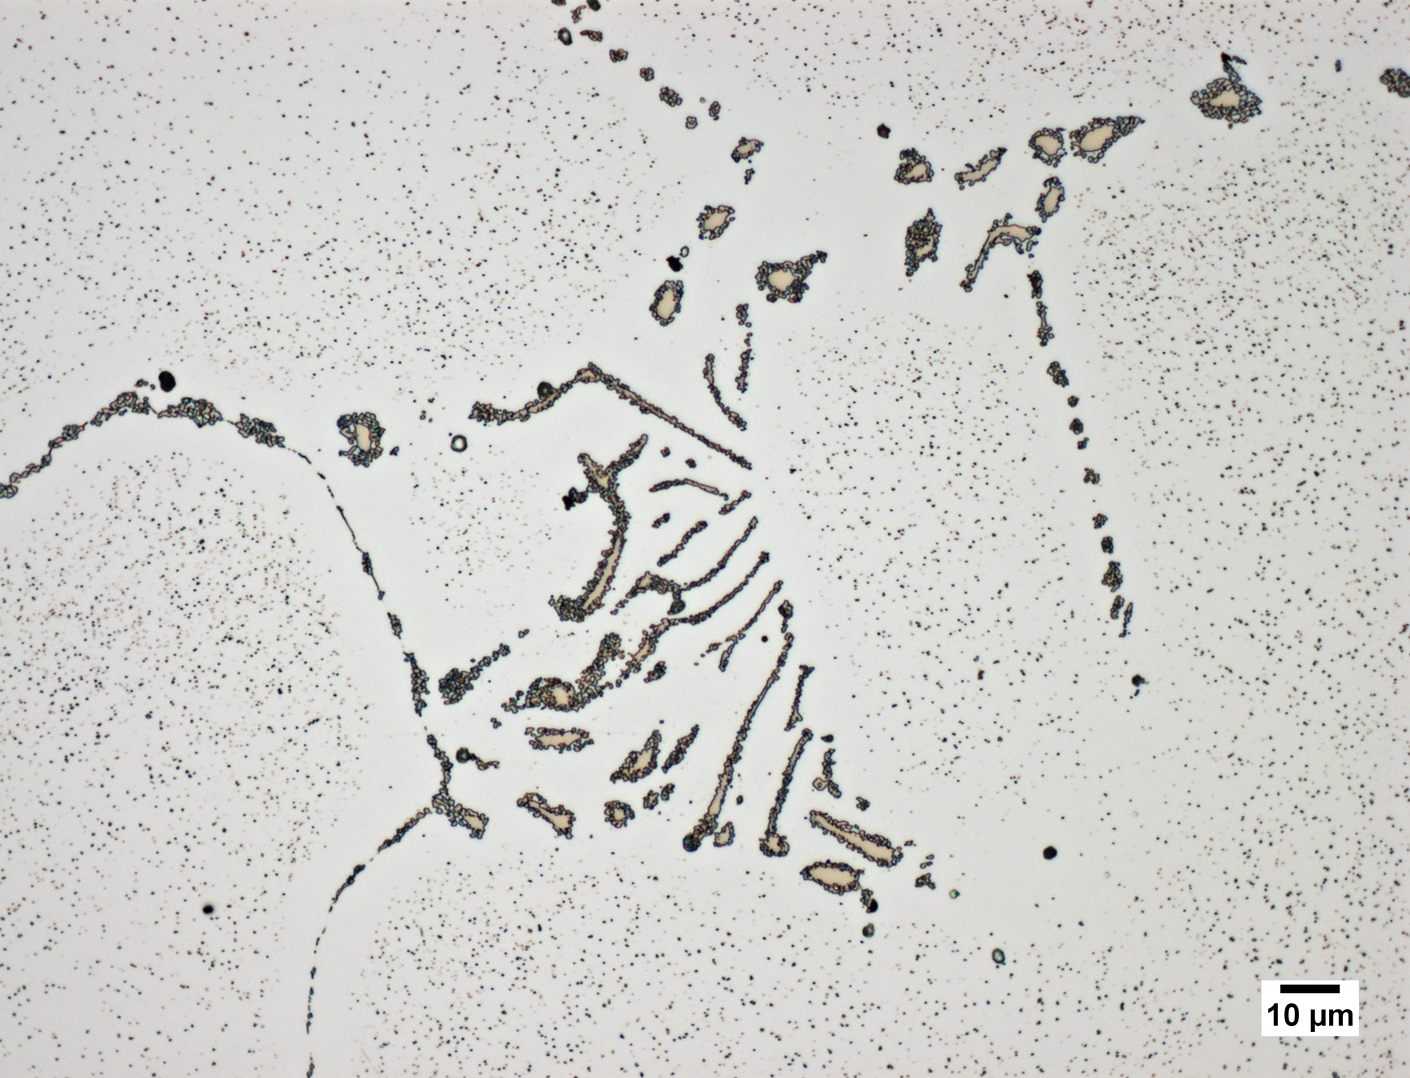
\includegraphics[width=4.7in]{figures/hot-ductility/c1-ar-500X}}
\caption[Optical Micrographs Showing the Typical As-Received Microstructure of Cone~1 Material.]{Optical Micrographs Showing the Typical As-Received Microstructure of Cone~1 Material (Service-Exposed) Utilized for Hot Ductility Testing, (A) 100X and (B) 500X.  Etch: 10\% Oxalic Acid, Electrolytic.}
\label{fig:c1-asreceived}
\end{figure}

\begin{figure}
\centering
\subfloat[100X]{\label{subfig:c5-asreceived-100X}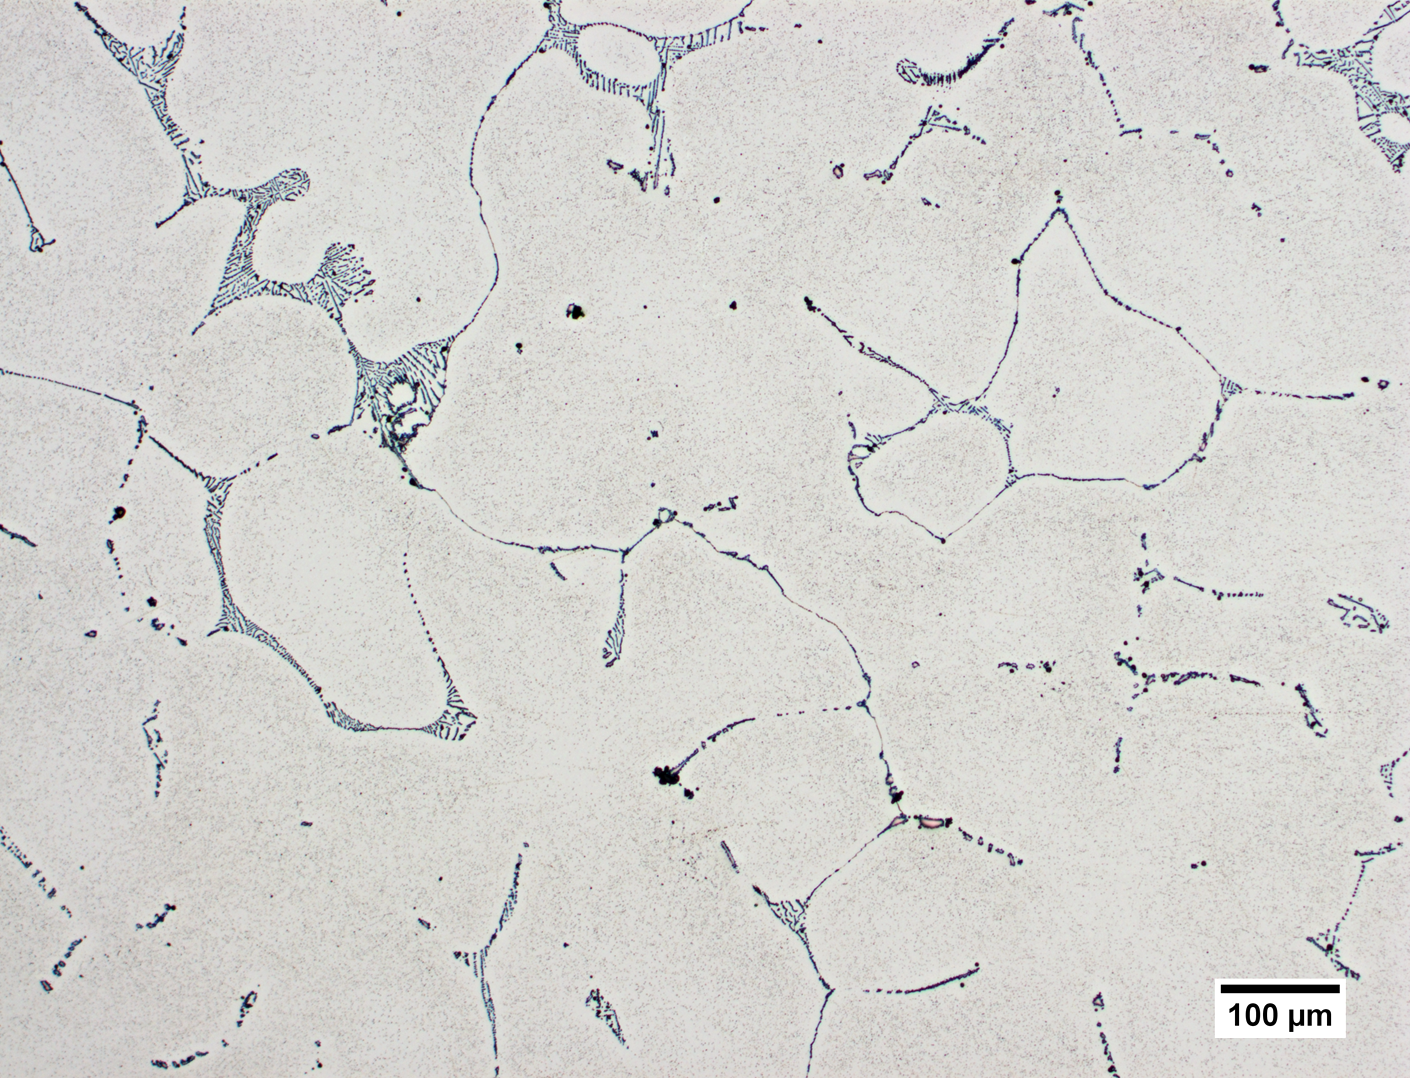
\includegraphics[width=4.7in]{figures/hot-ductility/c5-ar-100X}}

\subfloat[500X]{\label{subfig:c5-asreceived-500X}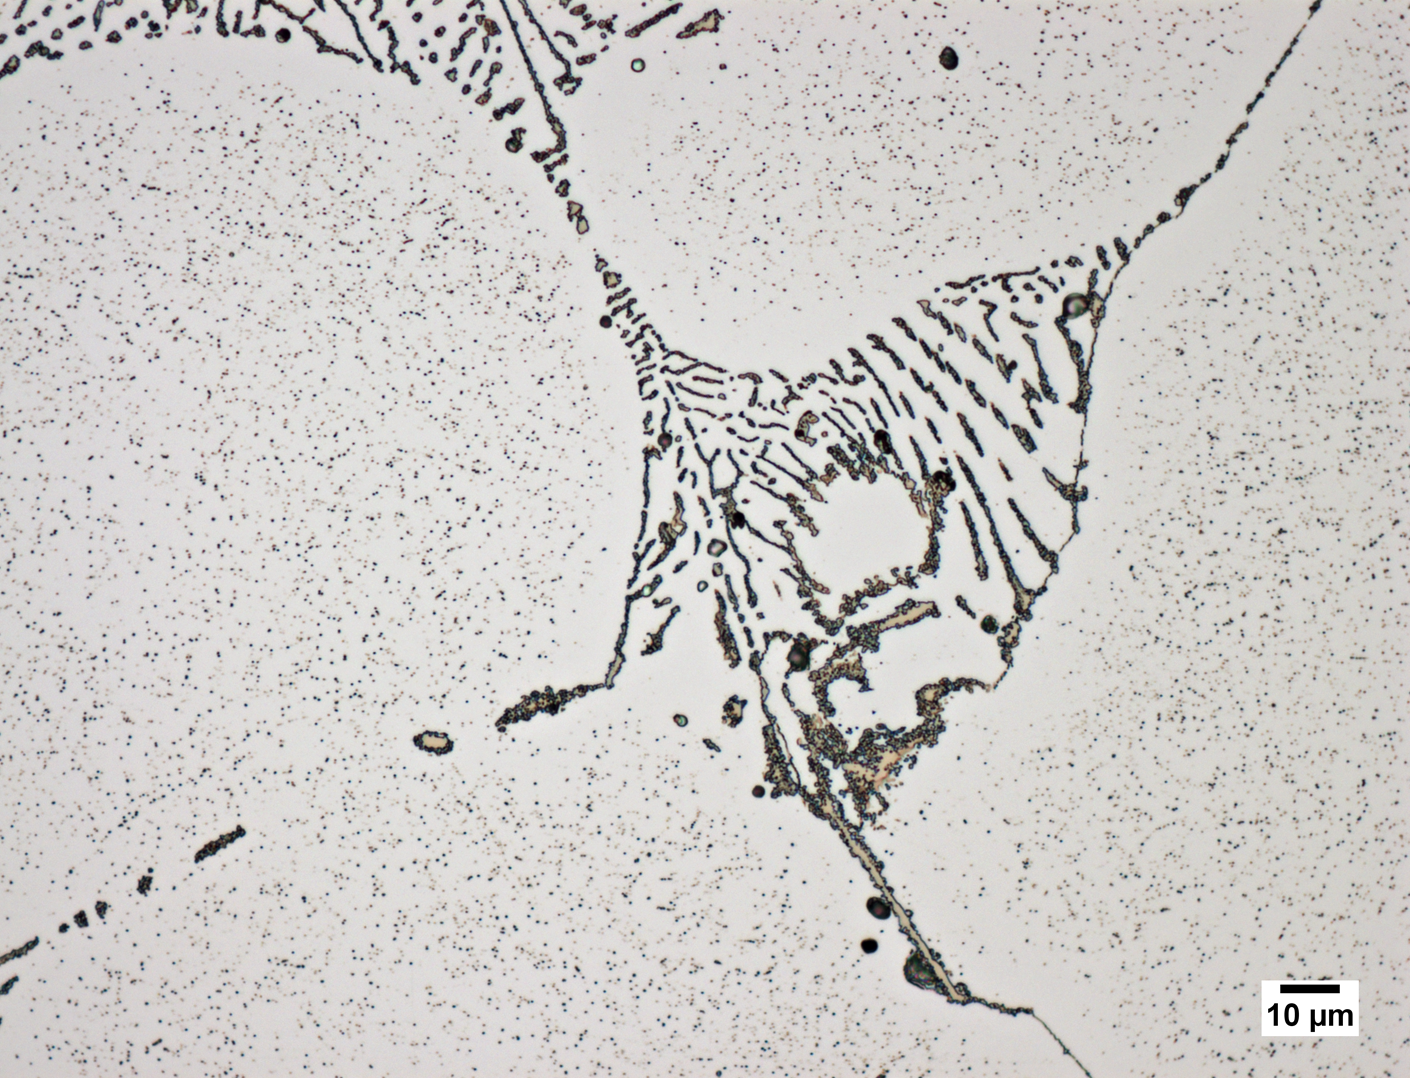
\includegraphics[width=4.7in]{figures/hot-ductility/c5-ar-500X}}
\caption[Optical Micrographs Showing the Typical As-Received Microstructure of Cone~5 Material.]{Optical Micrographs Showing the Typical As-Received Microstructure of Cone~5 Material (``Solution-Annealed'') Utilized for Hot Ductility Testing, (A) 100X and (B) 500X.  Etch: 10\% Oxalic Acid, Electrolytic.}
\label{fig:c5-asreceived}
\end{figure}


\begin{figure}
\centering
\subfloat[50X]{\label{subfig:c5-oh-2375-50X}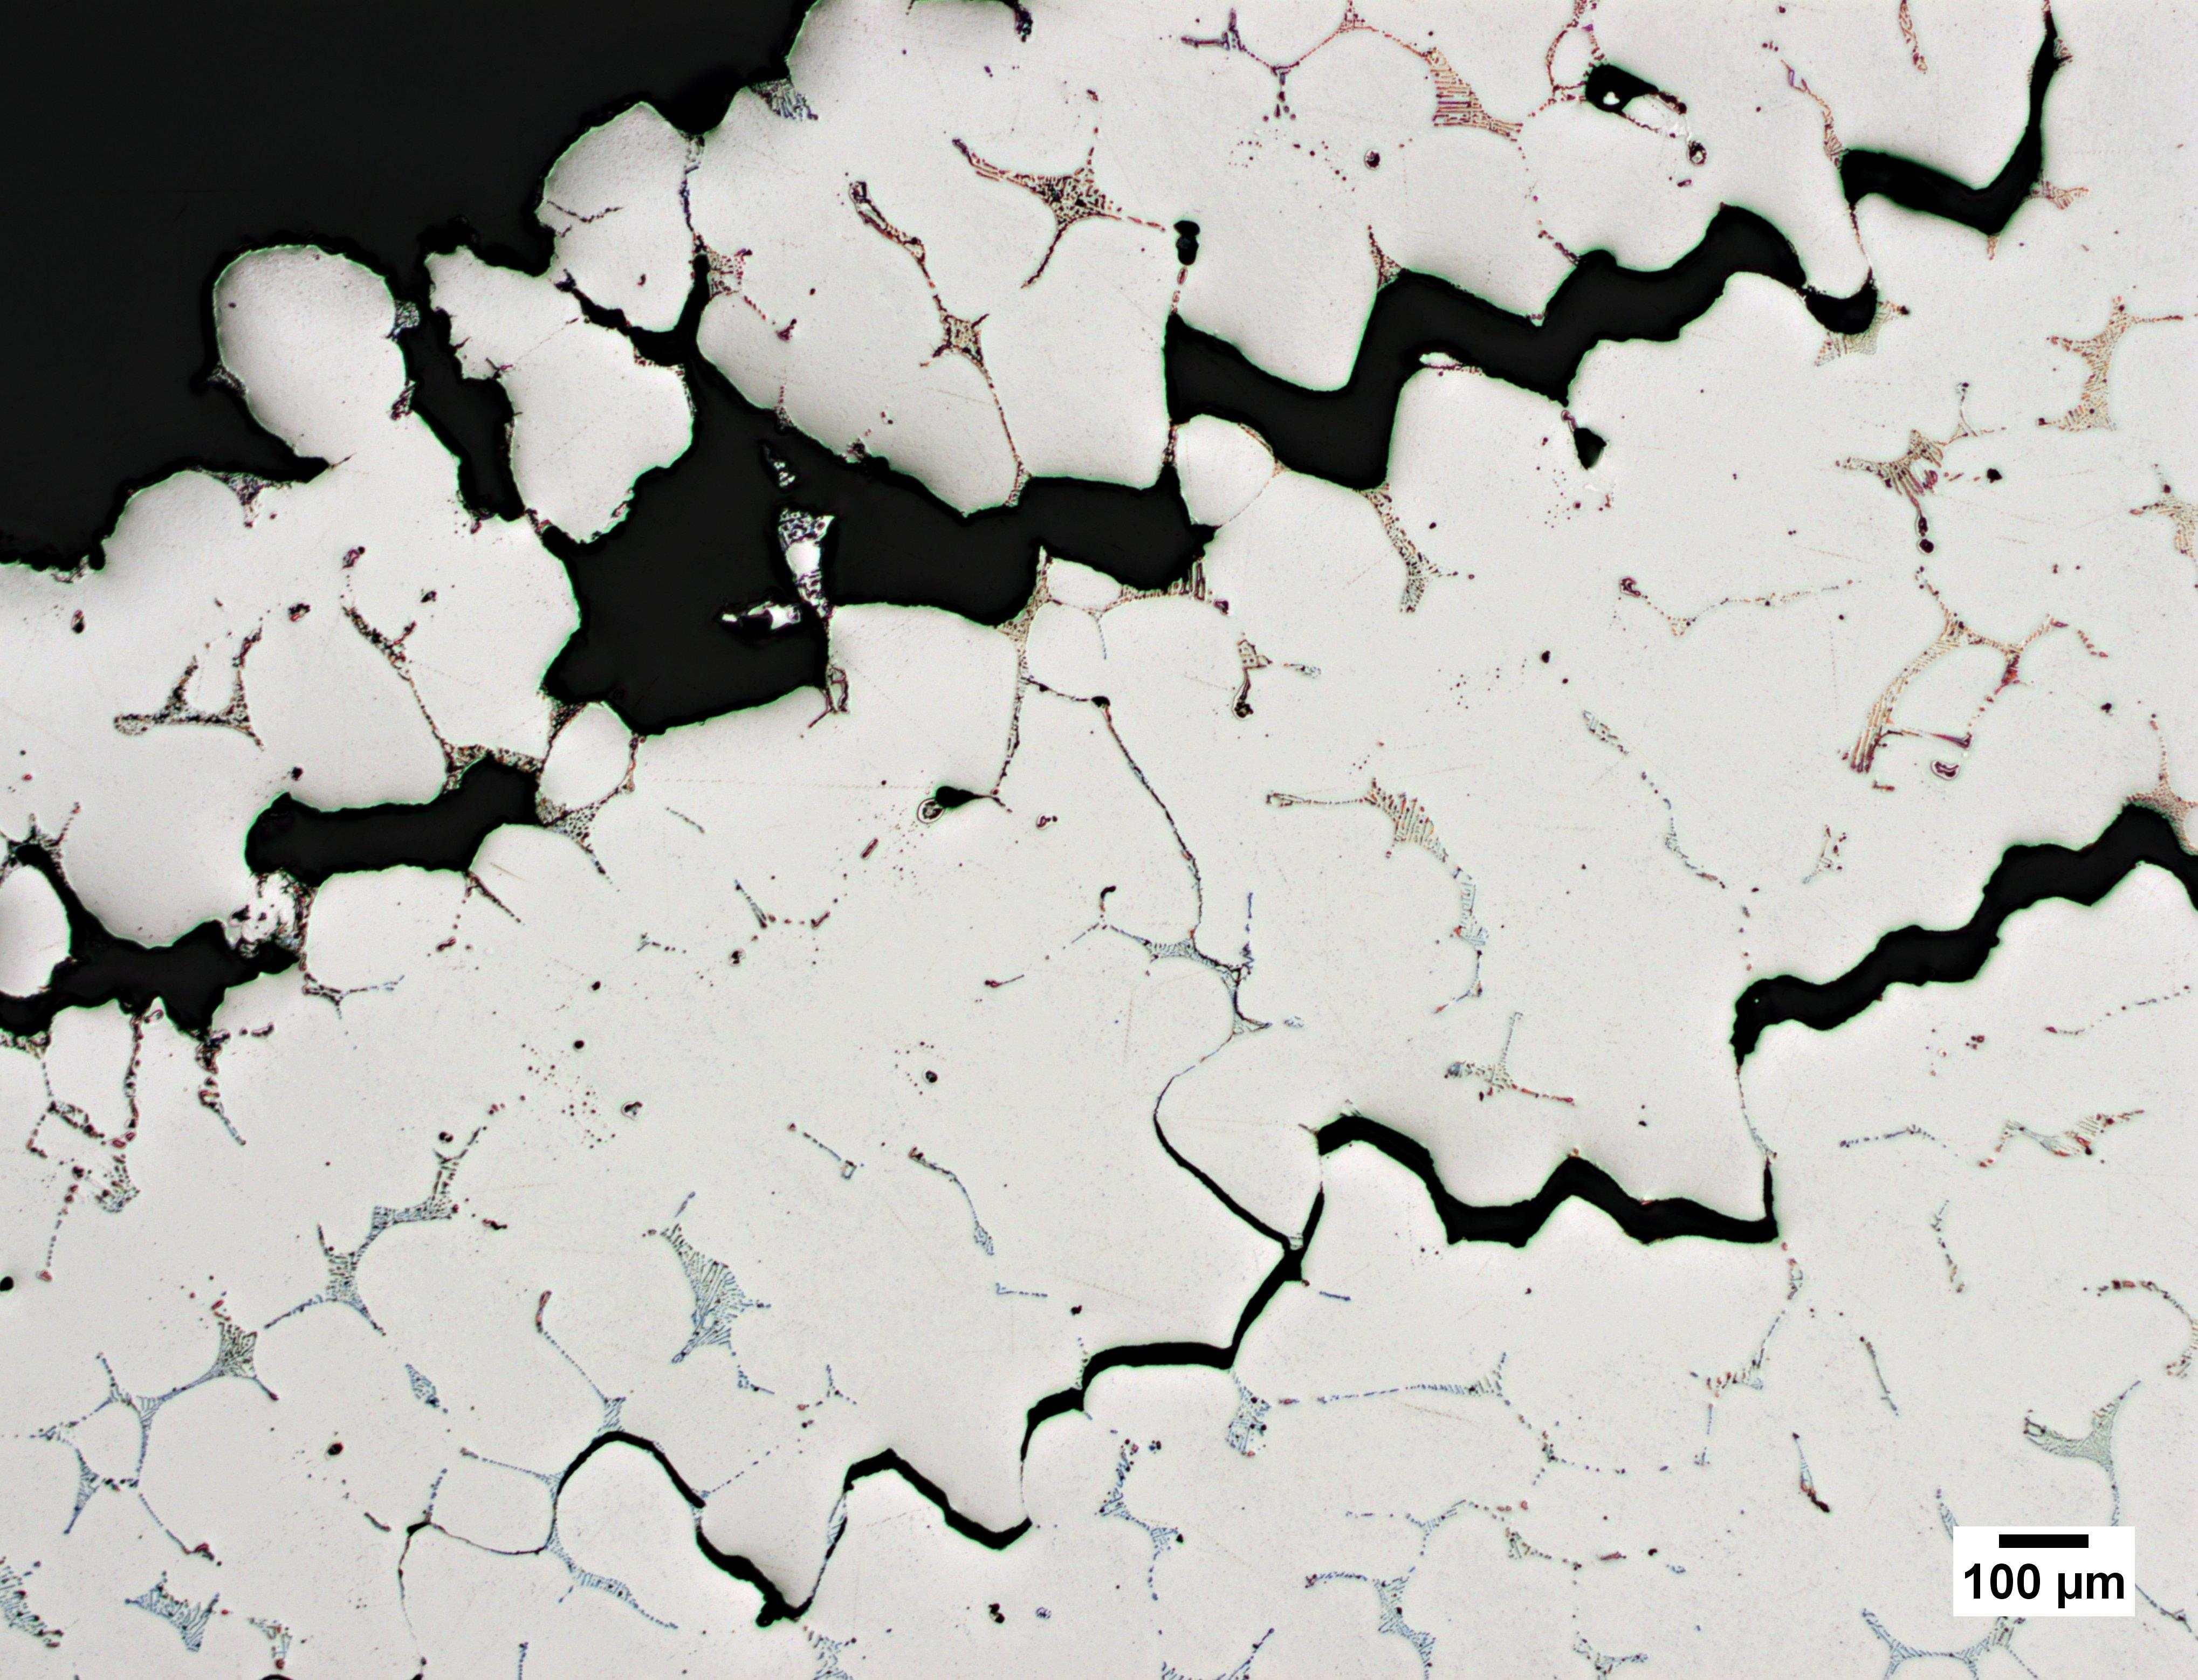
\includegraphics[width=4.7in]{figures/hot-ductility/c5-oh-2375-50x}}

\subfloat[200X]{\label{subfig:c5-oh-2375-200X}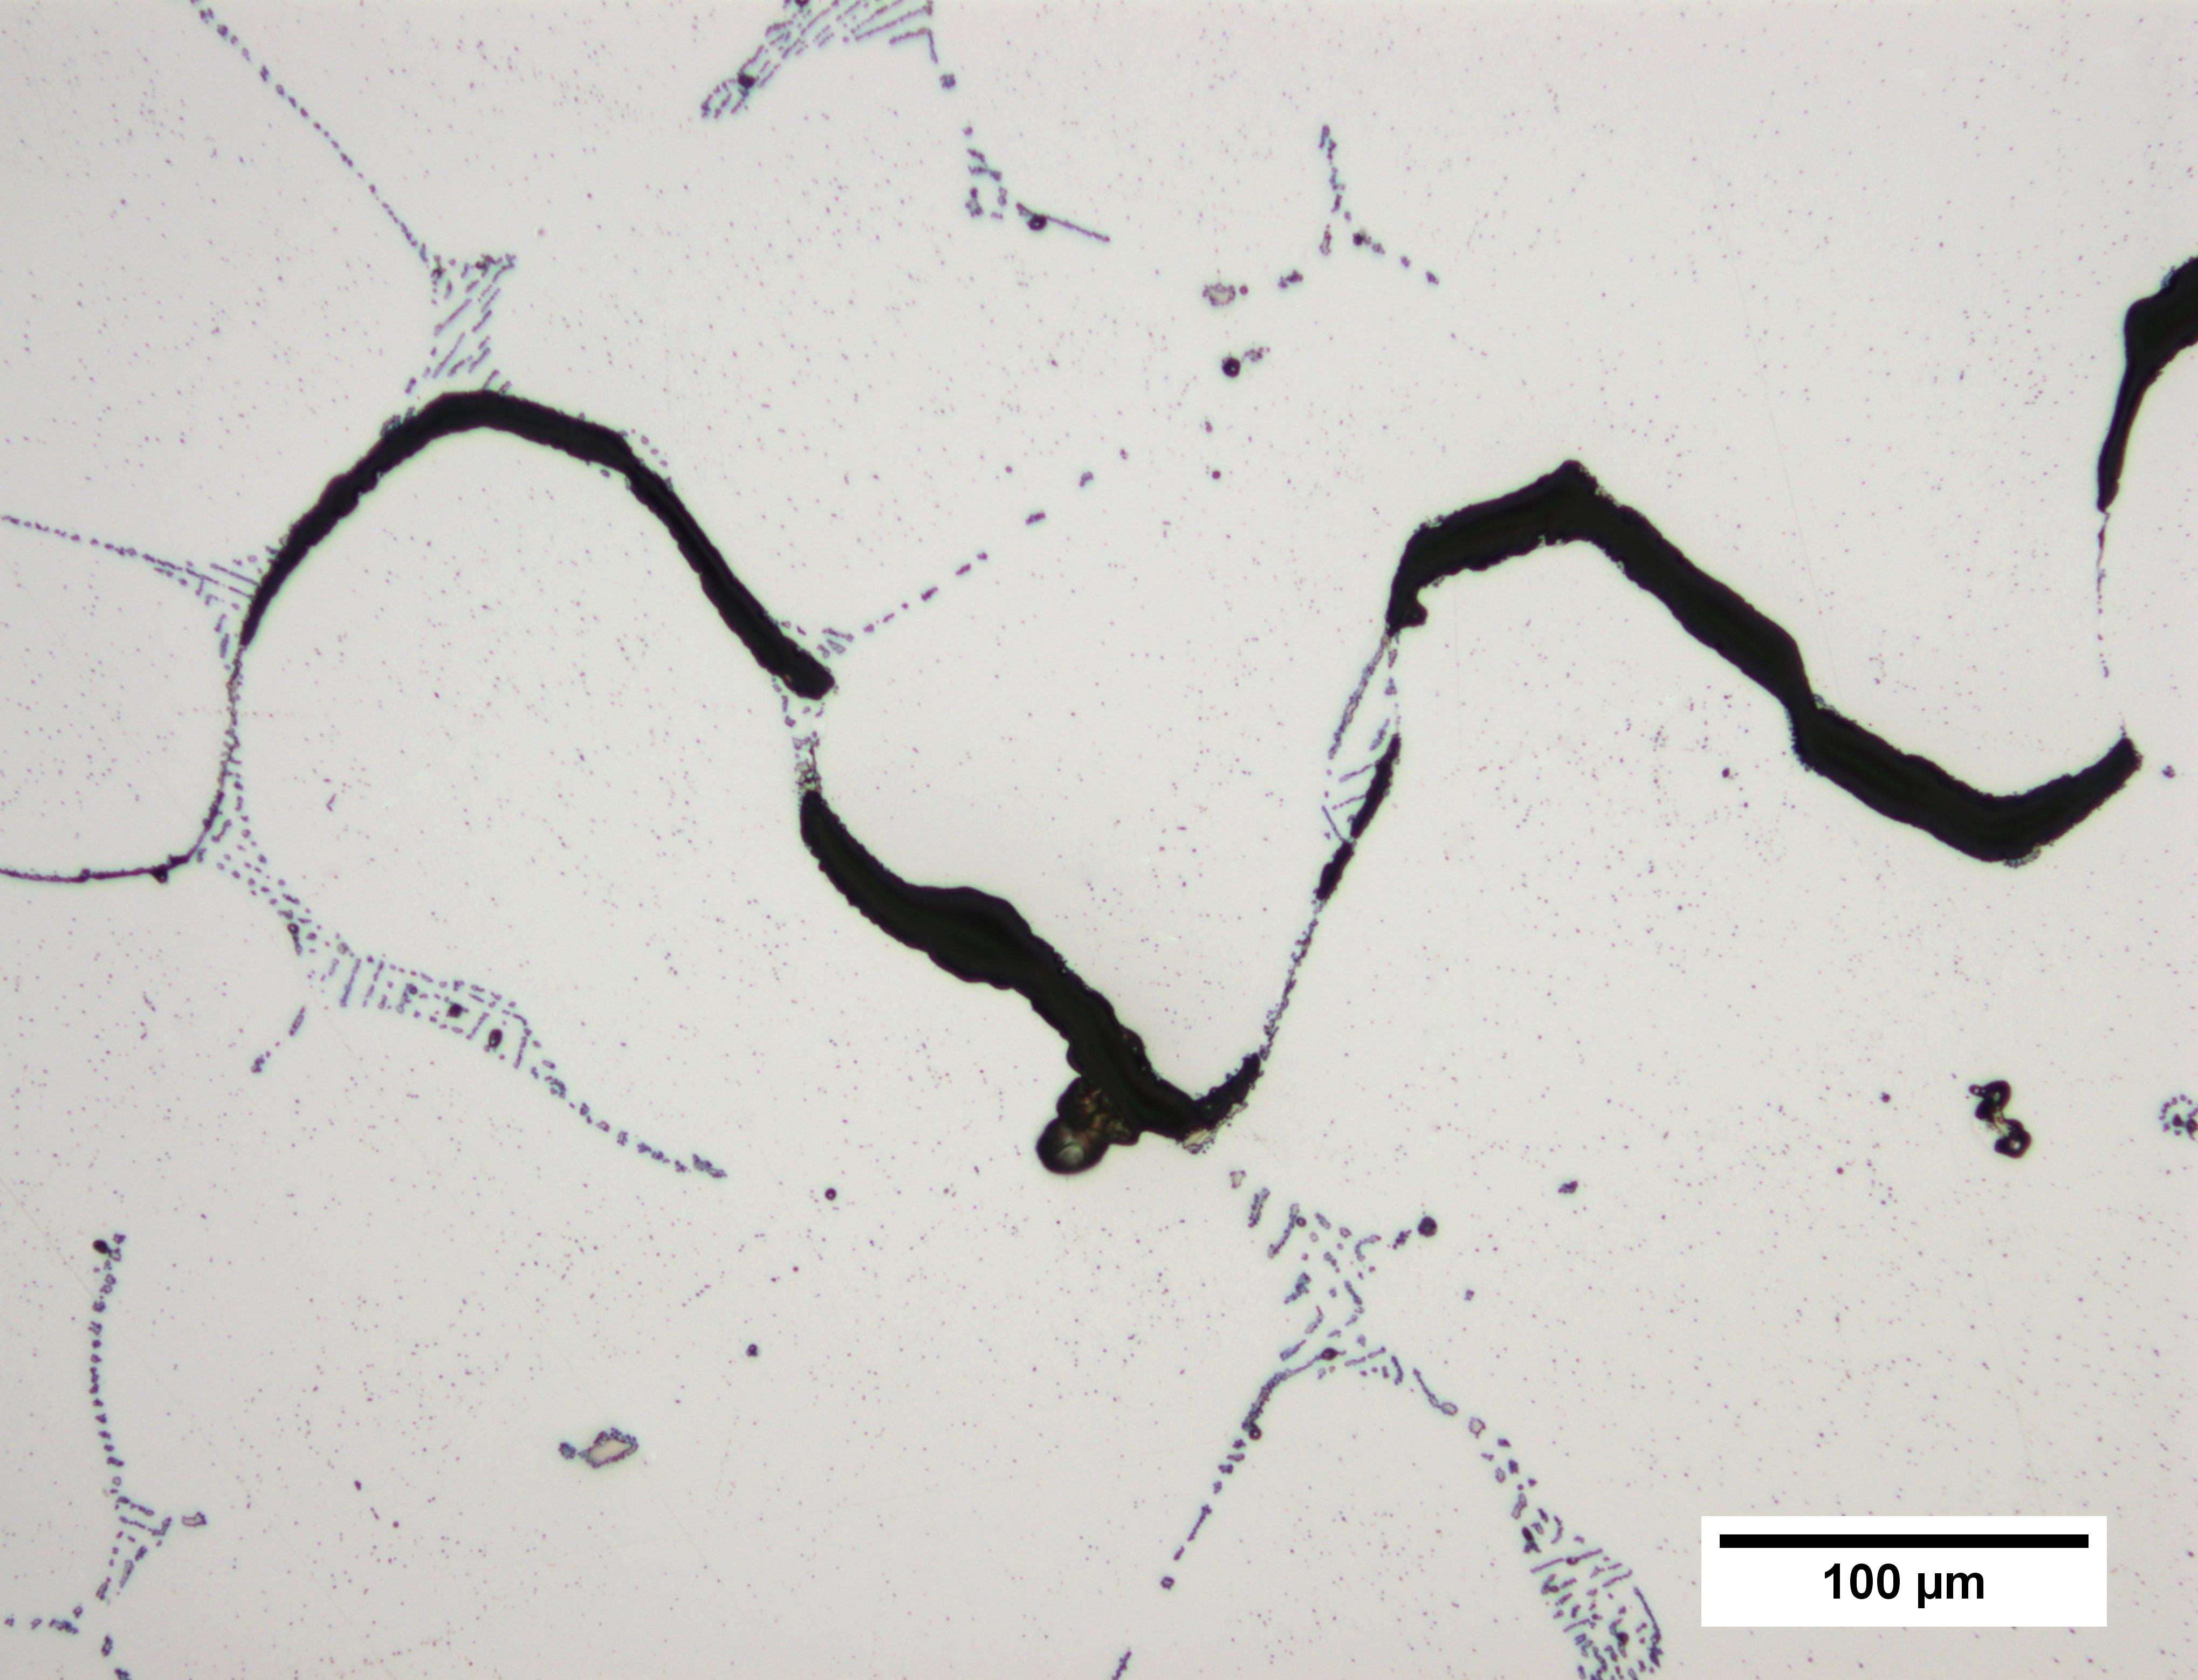
\includegraphics[width=4.7in]{figures/hot-ductility/c5-oh-2375-200x}}

\caption[Optical Micrographs Showing the Fracture Path as Revealed in a Longitudinal Section Through the Cone~5 2375\textdegree{}F On-Heating Hot Ductility Sample.]{Optical Micrographs Showing the Fracture Path as Revealed in a Longitudinal Section Through the Cone~5 2375\textdegree{}F On-Heating (\gls{zdt}) Hot Ductility Sample, at (A) 50X (B) 200X, (C) 500X and (D) 1000X.  Etch: 10\% Oxalic Acid, Electrolytic.}
\label{fig:c5-oh-2375}
\end{figure}


\begin{figure}
\ContinuedFloat
\centering
\subfloat[500X]{\label{subfig:c5-oh-2375-500X}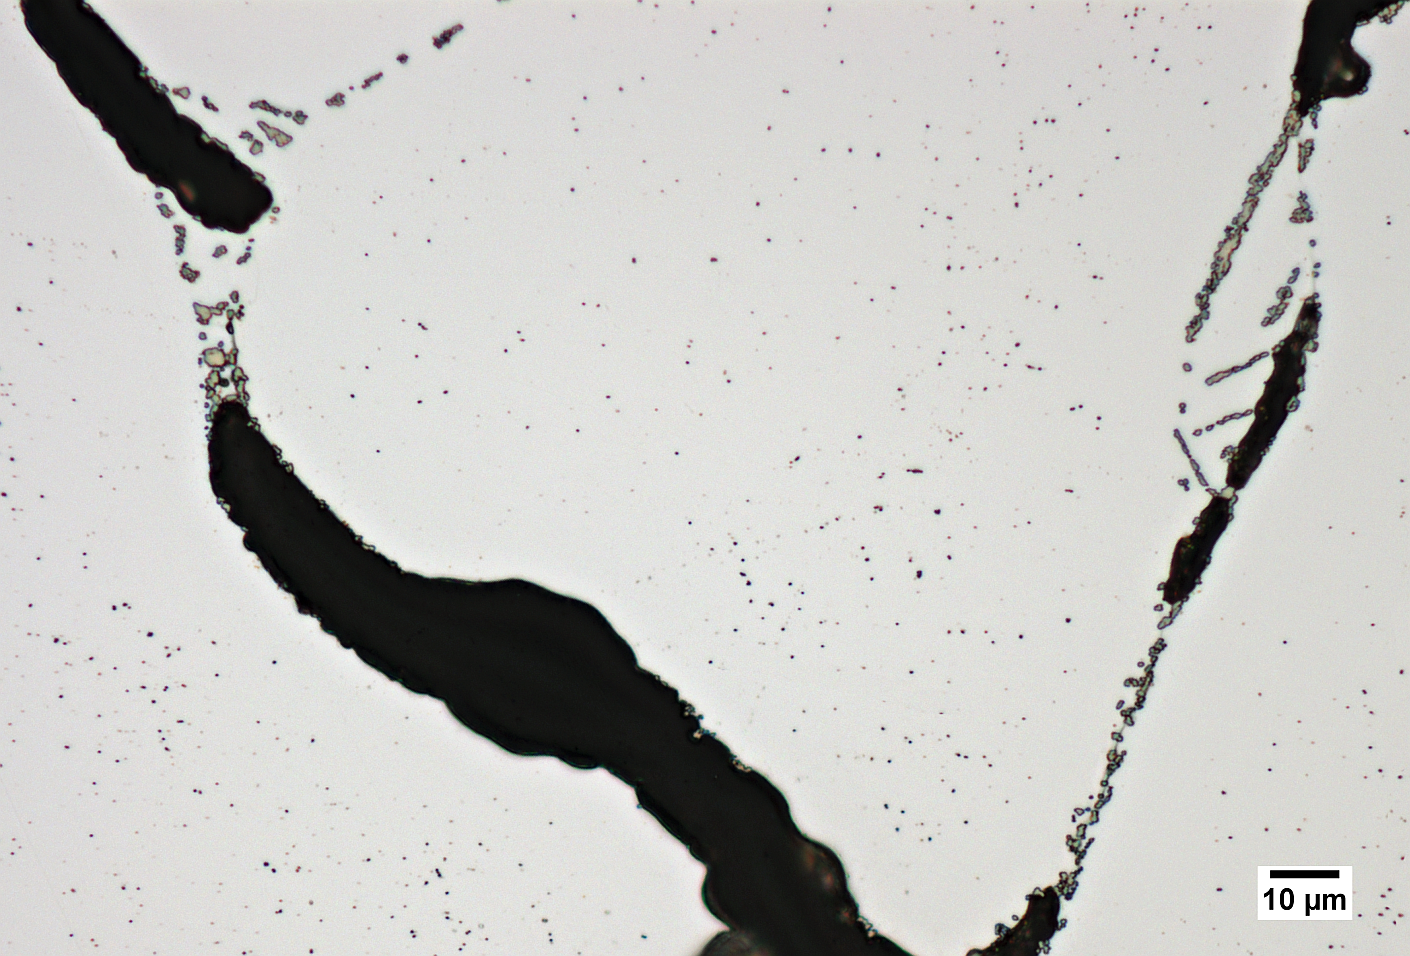
\includegraphics[width=4.7in]{figures/hot-ductility/c5-oh-2375-500x}}

\subfloat[1000X]{\label{subfig:c5-oh-2375-1000X}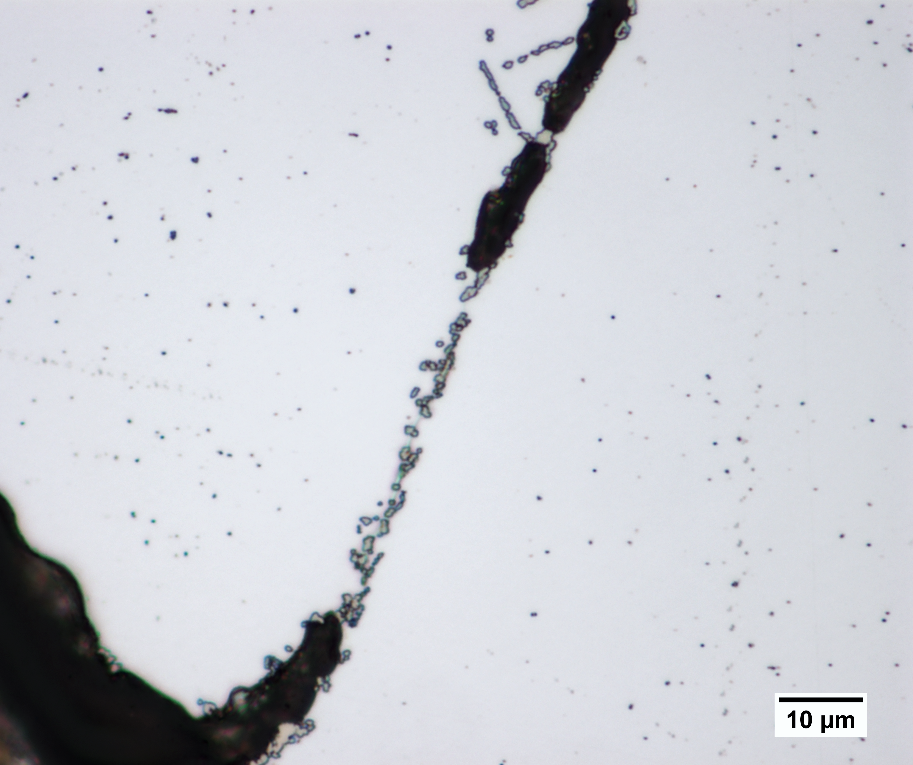
\includegraphics[width=4.7in]{figures/hot-ductility/c5-oh-2375-1kx}}
\caption[Optical Micrographs Showing the Fracture Path as Revealed in a Longitudinal Section Through the Cone~5 2375\textdegree{}F On-Heating Hot Ductility Sample.]{Optical Micrographs Showing the Fracture Path as Revealed in a Longitudinal Section Through the Cone~5 2375\textdegree{}F On-Heating (\gls{zdt}) Hot Ductility Sample, at (A) 50X (B) 200X, (C) 500X and (D) 1000X.  Etch: 10\% Oxalic Acid, Electrolytic.}

\end{figure}


\begin{figure}
\centering
\subfloat[200X]{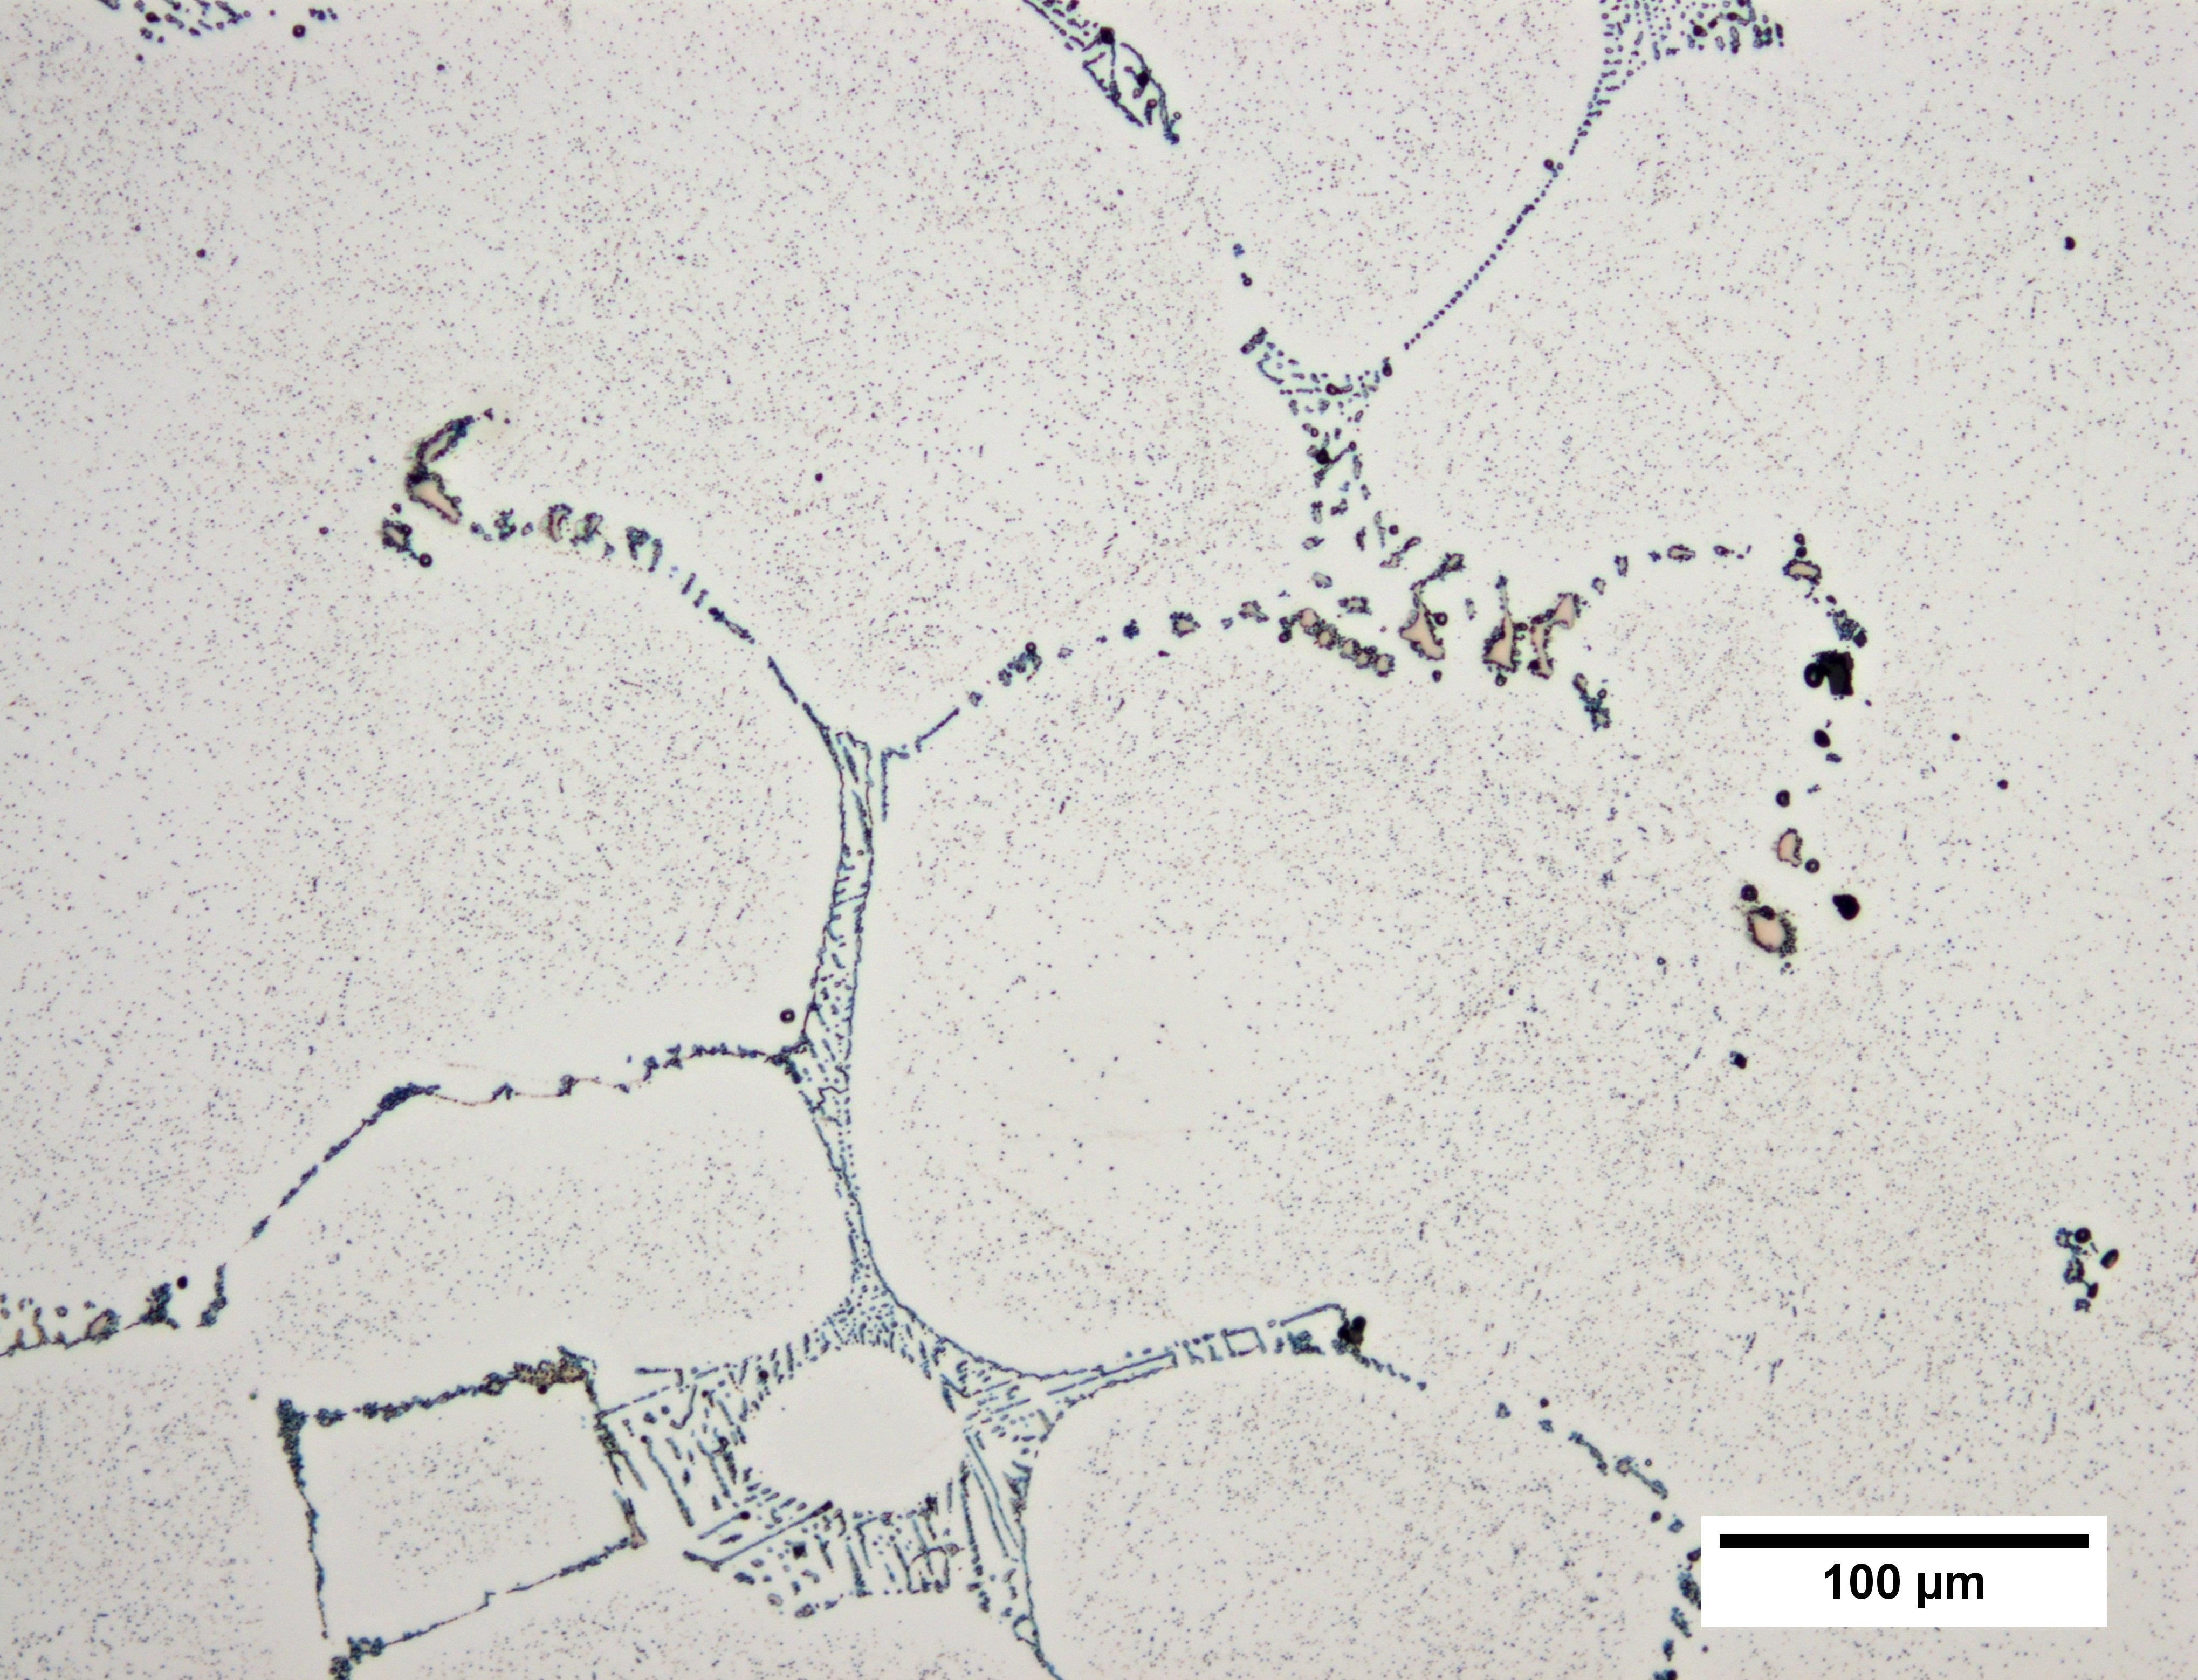
\includegraphics[width=4.7in]{figures/hot-ductility/c5-oh-2375-remote-200x}}

\subfloat[500X]{\label{subfig:c5-oh-2375-remote-500x}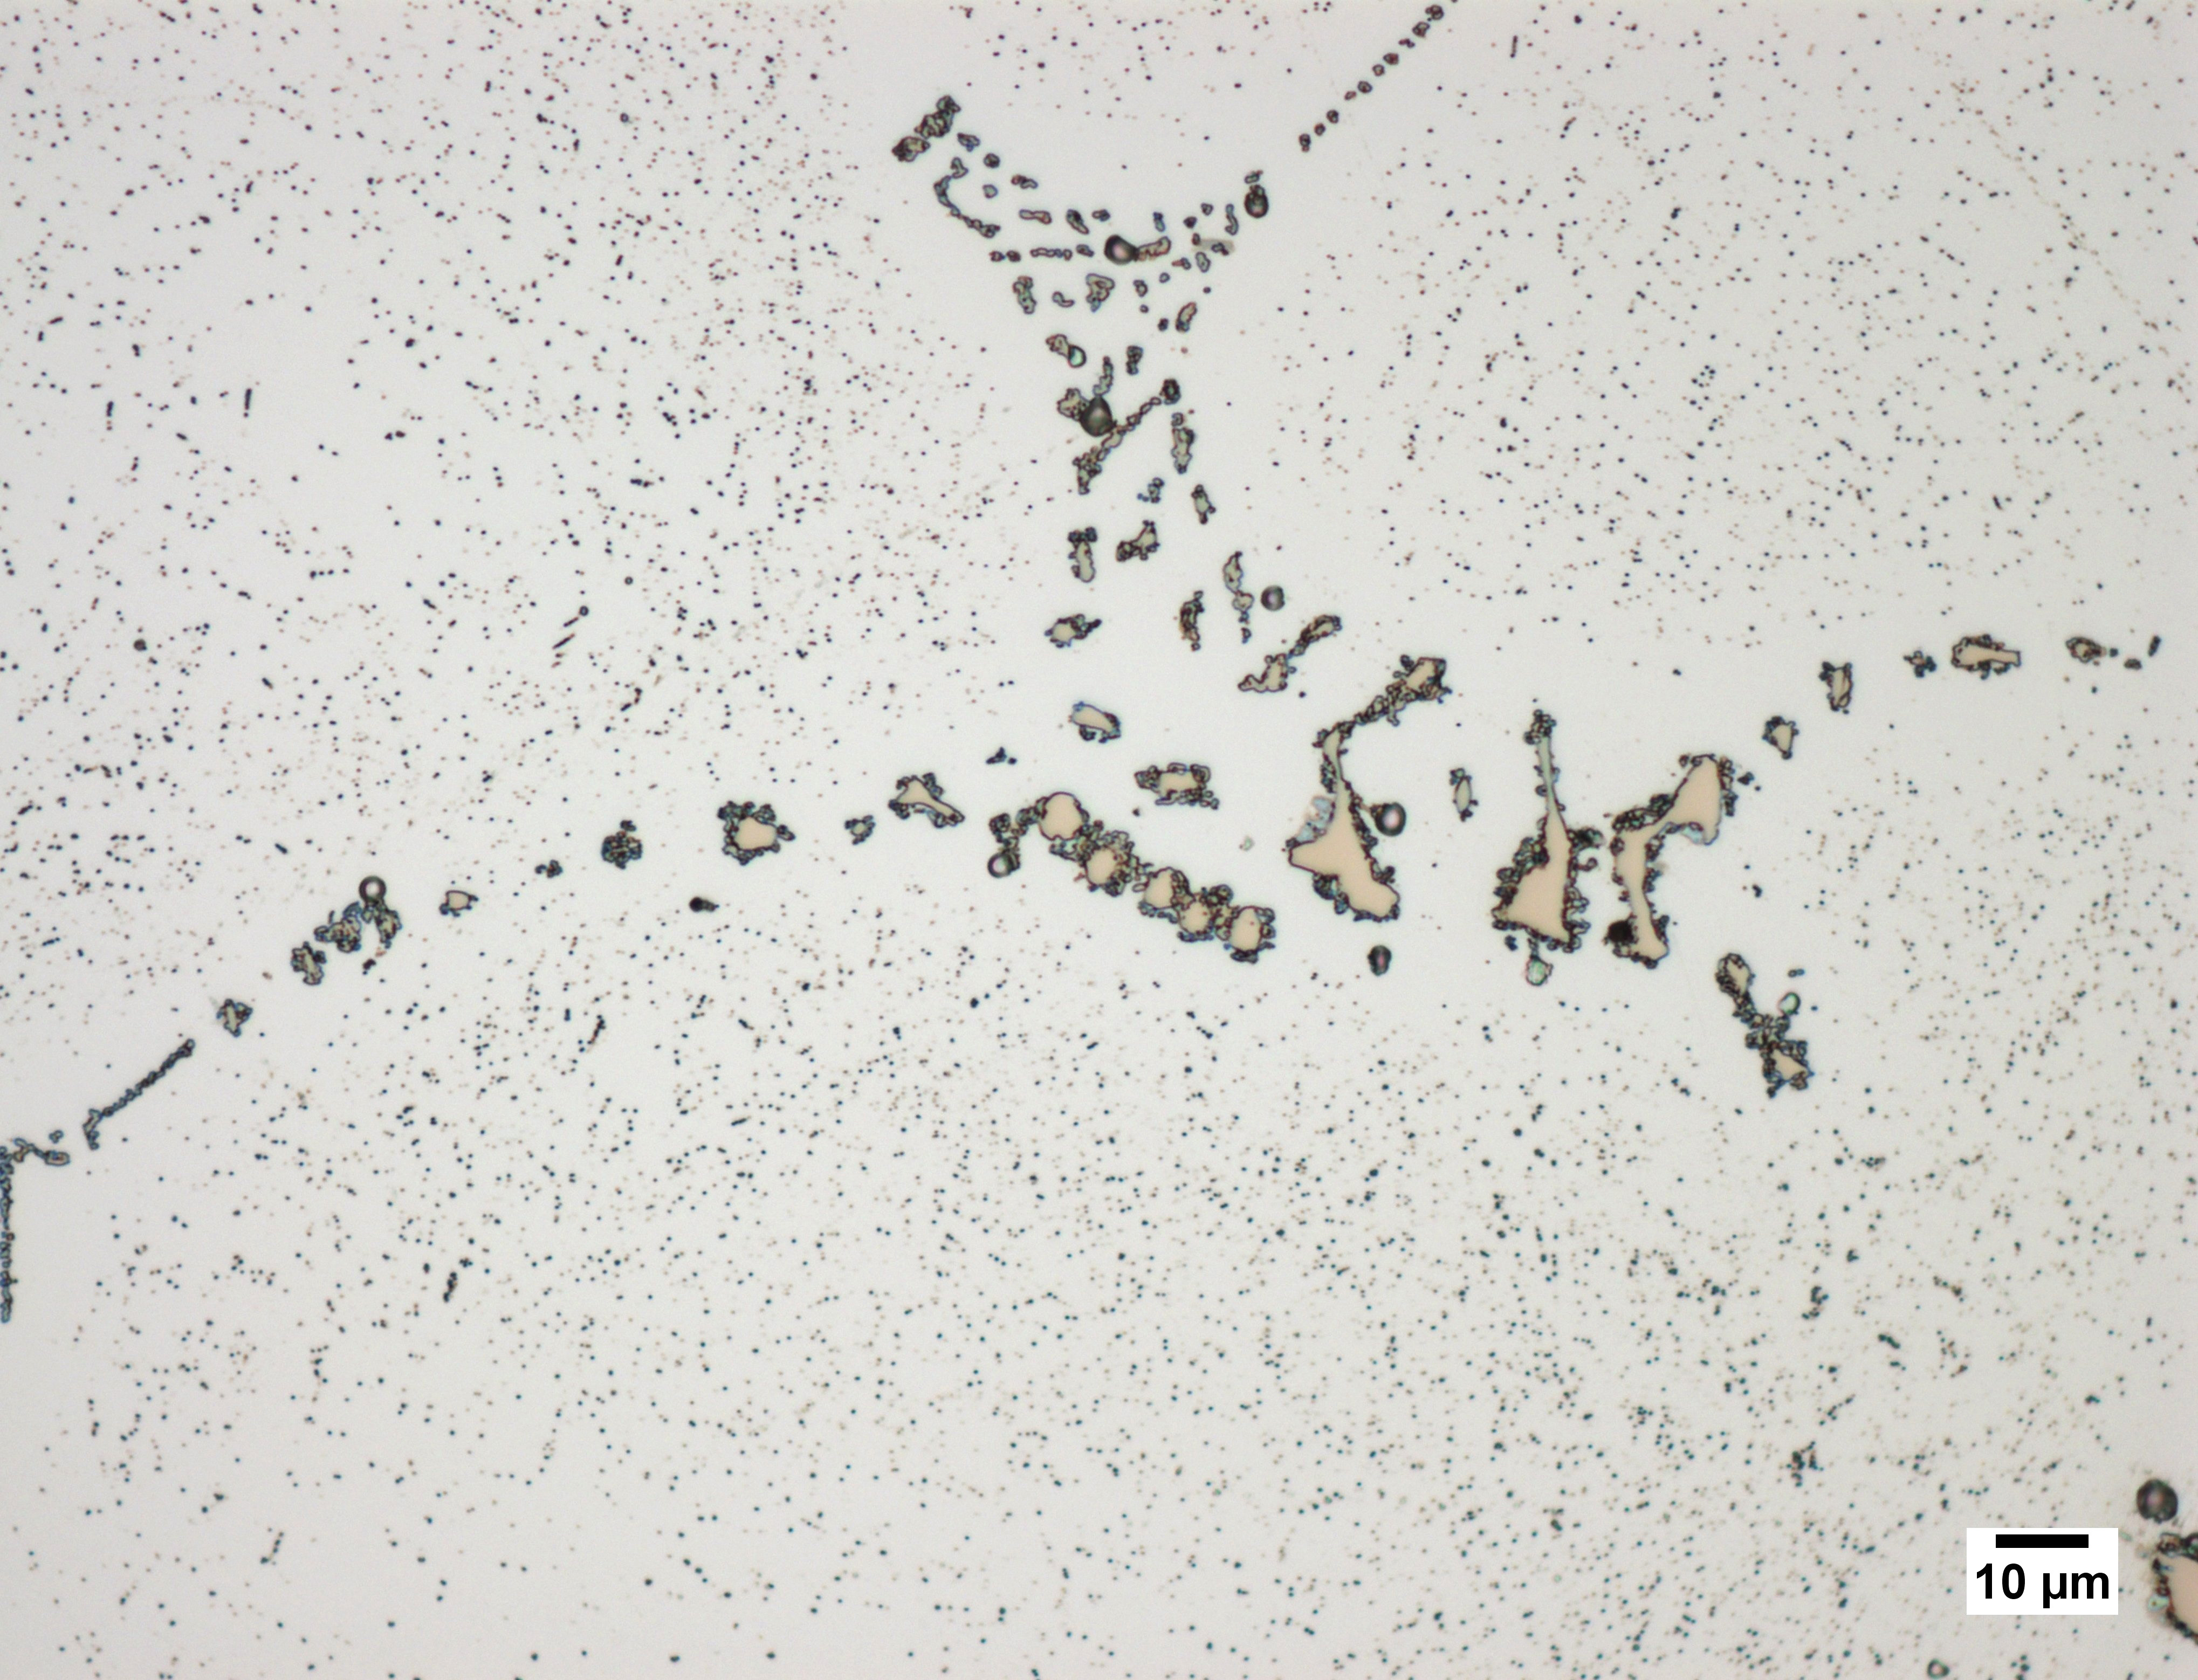
\includegraphics[width=4.7in]{figures/hot-ductility/c5-oh-2375-remote-500x}}

\caption{Optical Micrographs Showing the Microstructure of Unaffected Base Metal (Remote from the Fracture Location) in the Cone~5 2375\textdegree{}F On-Heating (\gls{zdt}) Hot Ductility Sample at (A) 200X and (B) 500X.  Etch: 10\% Oxalic Acid, Electrolytic.}
\label{fig:c5-oh-2375-remote}
\end{figure}

Comparing the micrographs shown in Figure 8 and Figure 9, it is apparent that the as-received Cone~1 and Cone~5 materials both exhibited a coarse dendritic microstructure with abundant intradendritic and interdendritic secondary phases.  Previous investigations (Hoffman and Colwell 1998; Hoffman and Gapinski 2001) of service-exposed 20Cr-32Ni-1Nb material with similar time in service indicated that the larger interdendritic phases were primarily niobium carbides (NbC), some of which were surrounded by a phase rich in Ni, Nb, and Si, while the intradendritic precipitates were determined to be mainly chromium carbides which precipitated as a result of service exposure.  The previously noted similarities in the hot ductility behavior are explained in light of the similarity of the as-received microstructures of the Cone~1 (``service-exposed'') and Cone~5 (``solution-annealed'') materials.  However, this was not the expected result based on the nominally reported material conditions since an earlier study on the repair weldability of 20Cr-32Ni-1Nb by Shi et al. (Shi, Lippold, and Ramirez 2010) indicated that solution annealed material showed a significantly different hot ductility response in terms of both on-heating and on-cooling behavior as compared to service-exposed material.  Therefore, the similar as-received microstructures of both Cone~1 and Cone~5, and the consequent similarities observed in the hot ductility characteristics, suggests that the weld joint region of Cone~5 (where the samples were extracted) was either not subjected to a solution annealing heat treatment or the parameters (temperature/time) were not adequate for an effective solution anneal, contrary to the information provided at the outset of this investigation.

Regarding the Cone~5 On-Heating 2375\textdegree{}F (ZDT) hot ductility sample, examination of Figure 10a indicates that regions near the fracture surface showed a noticeably reduced extent of matrix precipitates compared a region remote from the fracture surface  (Figure 11).  This reduction is due to the dissolution of precipitates as a result of the high temperature exposure from the simulated thermal cycle.  It is also apparent from Figure 10a that the crack paths proceed along the interdendritic boundaries; Figure 10c and Figure 10d show that the crack faces appear to be associated with the interdendritic secondary phases.  Cracking proceeds along these boundaries because they are the regions corresponding to the greatest degree of solute segregation and resulting formation of low-melting point constituents; consequently, melting will begin at these regions first during the high temperatures imposed during the simulated thermal cycle of the hot ductility test.  The identity of the interdendritic phases has not yet been verified but this will be pursued as part of the future work.
